\chapter{PACORA Implementation in a Manycore Operating System}
\section{Model Update and Downdate Algorithms}

\subsection{Row Update and Downdate}

Downdating makes an instructive example. A row downdate operation applies
a sequence of Givens rotations to the rows of $Q^T$.
The rotations are calculated to set every $Q^T_{i,dd}$, $i \neq dd$ to zero.
In the end only the diagonal element $Q^T_{dd,dd}$ of column $dd$ will be nonzero.
Since $Q^T$ remains orthogonal, the non-diagonal elements of row $dd$ will also have been zeroed automatically
and the diagonal element will have absolute value 1.
These same rotations are concurrently applied to the elements of $Q^T t$ and to the rows of $R$ $(= Q^T D)$
to reflect the effect that these transformations have on $Q^T$.

It is crucial to select pairs of rows and an order of rotations that preserves the upper triangular structure of $R$
while zeroing all but the diagonal entry of the chosen column $dd$ of $Q^T$.
Since $dd$ is always below the diagonal of $R$ it initially will contain only zeros.
It is therefore sufficient to rotate every non-$dd$ row with row $dd$, proceeding from bottom to top.
The first $m - n - 1$ rotations will keep row $R_{dd,*}$ entirely zero,
and the remaining $n$ rotations will introduce nonzeros in $R_{dd,*}$ from right to left.
The effect on $R$ will be to replace zero elements by nonzero elements only within row $dd$.
At this point, except for a possible difference in overall sign, $R_{dd,*} = D_{dd,*}$.

Now the rows from 0 down through $dd$ of the modified matrices $Q^Tt$ and $R$ and both the rows and columns of the modified $Q^T$
are circularly shifted by one position, moving row $dd$ to the top (and column $dd$ of $Q^T$ to the left edge).
The following is the result:
\begin{displaymath}
\begin{array}{lll}
    \left[\begin{array}{cc}
      \pm1  &  0 \\
      0     &  \tilde{Q}^T
   \end{array}\right]
   \left[\begin{array}{c}
      t_{dd} \\
      \tilde{t}
   \end{array}\right]
   &=&
   \left[\begin{array}{c}
      \pm D_{dd,*} \\
      \tilde{R}
   \end{array}\right] w
   \\
   \\
   &-&
   \left[\begin{array}{cc}
      \pm1  &  0 \\
      0     &  \tilde{Q}^T
   \end{array}\right]
   \left[\begin{array}{c}
      \varepsilon_{dd} \\
      \tilde{\varepsilon}
   \end{array}\right]
\end{array}
\end{displaymath}
The top row has thus been decoupled from the rest of the factorization and may either be deleted or updated with new data.

The update process more or less reverses these steps, adding a new top row to $R$ and $t$ and a row and column to $Q^T$.
Then $R$ is made upper triangular once more by a sequence of Givens rotations that zero its sub-diagonal elements
(formerly the diagonal elements of $\tilde{R}$) one at a time.
These rotations are applied not just to $R$ but also to $Q^Tt$ and of course to $Q^T$ itself.

\subsection{Rank Preservation}

Deciding in advance whether downdating a row of $R$ will reduce its rank
is equivalent to predicting whether one of the Givens rotations, when applied to $R$,
will zero or nearly zero a diagonal entry of $R$.
This is particularly easy to discover because $dd$, the row to be downdated, is initially all zeros in $R$,
\emph{i.e.} in the lower part of the matrix.
In this situation a diagonal entry of $R$, $R_{i,i}$ say, will be compromised if and only if the
cosine of the Givens rotation that involves rows $dd$ and $i$ is nearly zero.
The result will be an interchange of the zero in $R_{dd,i}$ with the nonzero diagonal element $R_{i,i}$.
$R_{dd,i}$ is zero before the rotation because
$R$ was originally upper triangular and prior rotations only involved row subscripts greater than $i$.

\pacora keeps track of the sequence of values in $Q^T_{dd,dd}$ without actually changing $Q^T$
so that if the downdate at location $dd$ is eventually aborted there is nothing to undo.
It is also possible to remember the sines and cosines of the sequence of rotations
so they don't have to be recomputed if success ensues.
A rank-preserving row to downdate will always be available as long as $R$ is sufficiently ``tall''.
Having at least twice as many rows as columns is enough since the number of available rows to downdate
matches or exceeds the maximum possible rank of $R$.

\subsection{Column Update and Downdate}

The active-set NNLS method is based on the idea that since the only constraints are variable positivity
then for all components either the variable or its gradient will be zero at a solution point; see~\cite{BoVa}, page~142.
The active set, denoted by \textbf{Z}, comprises the column subscripts $j$ for which the variable $w_j$ is zero and the gradient $v_j$ is positive. If a column $j$ not currently in \textbf{Z} happens to acquire a negative $w_j$ after a back-solve, $w_j$ is zeroed,
$j$ is moved into \textbf{Z} and column $j$ is downdated in $R$, thereby making the gradient positive.
Conversely, if a column already in \textbf{Z} happens to acquire a negative gradient $v_j$ it is removed from \textbf{Z} and updated in $R$,
allowing it to further reduce the value of the objective function.

After initial acquisition of data and $QR$ factorization, each step of \pacora's NNLS algorithm
combines incremental row and column downdates and updates as follows:

\begin{pseudocode}{IncrementalNNLS}{t_0,d_0}
\LOCAL{R,Q^T,Q^Tt,w,v,idx,d,u,done}                              \\
R,Q^T,Q^Tt \GETS \textsc{DndtRow}(R,Q^T,Q^Tt,idx)           \\
R,Q^T,Q^Tt \GETS \textsc{UpdtRow}(t_0,d_0,R,Q^T,Q^Tt,idx)     \\
w \GETS \textsc{BackSolve}(R,Q^Tt,idx)                          \\
v \GETS \textsc{Gradient}(R,Q^Tt,idx)                    \\
\REPEAT
  done \GETS \TRUE                                              \\
  d \GETS \arg\min(w)                                          \\
  \IF w_d < 0 \THEN                                            \\
  \BEGIN
    done \GETS \FALSE                                         \\
    R,Q^T,Q^Tt,idx \GETS \textsc{DndtCol}(R,Q^T,Q^Tt,idx,d)   \\
    w \GETS \textsc{BackSolve}(R,Q^Tt,idx)                    \\
    v \GETS \textsc{Gradient}(R,Q^Tt,idx)              \\
  \END                                                        \\
  u \GETS \arg\min(v)                                         \\
  \IF v_u < 0 \THEN                                           \\
  \BEGIN
    done \GETS \FALSE                                         \\
    R,Q^T,Q^Tt,idx \GETS \textsc{UpdtCol}(R,Q^T,Q^Tt,idx,u)     \\
    w \GETS \textsc{BackSolve}(R,Q^Tt,idx)                    \\
    v \GETS \textsc{Gradient}(R,Q^Tt,idx)              \\
  \END                                                        \\
\UNTIL done                                                   \\
\RETURN{w,v}                                                  \\
\end{pseudocode}

The set \textbf{Z} and its complement \textbf{P} are implemented as an index $idx$
containing a vector of the column subscripts comprising \textbf{P} in increasing order
followed by the column subscripts of \textbf{Z} in increasing order;
$idx$ also contains an offset defining the beginning of \textbf{Z} in the vector.
For example, if columns 1, 3, and 4 are in \textbf{Z} and columns 0, 2, and 5 are in \textbf{P}
then the resulting vector is [0 2 5 1 3 4] and the offset is 3.
Since the offset is just the size of the set \textbf{P} it is naturally called $p$.

Regaqrdless of status, columns are left in place in $R$
The columns of $R$ belonging to \textbf{P} are denoted by $R^p$ and those in \textbf{Z} by $R^z$.
The updating or downdating of a column only involves modifying the index $idx$ to redefine \textbf{P} and \textbf{Z} and then
applying Givens rotations to the rows of $R$ to restore $R^p$ to upper triangular form.

When a column indexed by $d$ in $R^p$ is downdated because $w_d < 0$, that column is moved from \textbf{P} to \textbf{Z} in $idx$.
To restore $R^p$ to upper triangular form, Givens rotations are applied to $R$ at rows $R_{d,*}$ and $R_{k,*}$
where $d < k < p$. The row subscripts $k$ are used in decreasing order from $p-1$ down to $d+1$,
and each rotation zeros the subdiagonal element in $R^p$ of the column indexed by $k$.
As usual, these rotations are also applied to $Q^T$ and $Q^Tt$.
The result in $R^z$ is a ``spike'' of nonzeros in the column that was moved;
it can eventually extend to the bottom of $R$ as \emph{row} updates occur.

Column movements from \textbf{Z} to \textbf{P} are based on the gradient $v$ of the objective function, namely
\begin{eqnarray*}
v &=& 1/2\nabla\|Dw - t\|^2_2 \\
  &=& D^T(Dw - t)             \\
  &=& R^TQ^T(QRw - t)         \\
  &=& R^T(Rw - Q^Tt)          \\
  &=& R^T(-Q^T\varepsilon).
\end{eqnarray*}
If for some column in \textbf{Z} the inner product of the corresponding spiked row in $R^T$ and $-Q^T\varepsilon$ is negative,
the column subscript must be moved to \textsc{P}.
Updating $R^p$ reverses the downdating steps by zeroing the spike via a sequence of Givens rotations on $R$
between adjacent pairs of rows, starting at the bottom and ending at $m,m+1$ where $m$ is the position of the new column in $idx$.
These rotations conveniently extend the columns to the right of $m$ in $R^p$ by one,
thus restoring $R^p$ to upper triangular form. Once again, the rotations are also applied to $Q^T$ and $Q^Tt$.

A new gradient computation and new back-solve for $w$ are clearly necessary after either downdates or updates to columns of $R$.



\section{Dynamic Penalty Optimization}\label{dyn_opt}

%IV.	Dynamic Optimization
%	a.	Gradient Descent w/ Backtracking Search
%		i. boundary conditions clean up
%	b.	Dealing with Fractional Results

\pacora's penalty optimization algorithm dynamically decides resource allocations. The algorithm can be run periodically, when applications start or stop, when an application changes phase or when the system changes operating scenarios.  One of the advantages of convex optimization is that it enables fast, incremental solutions.  As shown in our experiments, the algorithm can terminate earlier to decrease overhead and still be moving towards an optimal solution as it runs.  %However we found in our implementation that the algorithm was fast enough to run to completion every time. 

Convex optimization is simplest when it is unconstrained, so we reformulated \pacora's construction to be unconstrained.
Extending the response time model functions to all of $\Re^n$
moves the requirement that allocations must be positive into the objective function,
and introducing application 0 for slack resources turns the affine inequalities into equalities:
\begin{eqnarray*}
& \makebox[1in][r]{Minimize}   & \sum_{p\in P} {\pi_p(\tau_p(a_{p,1}\ldots a_{p,n}))}  \\
& \makebox[1in][r]{Subject to} & \sum_{p\in P} a_{p,r} = A_r, r = 1,\ldots n           \\
\end{eqnarray*}

The only remaining constraints are those on the $a_{p,r}$.
These can be removed by letting the $a_{p,r}$ be unbounded above for $p \neq 0$
and changing the domain of $\tau_0$  to be the whole resource allocation matrix.
The definition of $\tau_0$ might take the form
\begin{eqnarray*}
\tau_0 &=& \sum_r \Delta_r \sum_{p \neq 0} a_{p,r}     \\
       &=& \sum_r \Delta_r (A_r - a_{0,r})
\end{eqnarray*}
where $\Delta_r$ is the (constant) power dissipation of one unit of resource $r$.
However, if any of the allocations $a_{0,r}$ turns out to be negative then $\tau_0$  should instead return the value $+\infty$.
%This modification of the objective function transforms the resource allocation problem
%to unconstrained convex optimization.  

The penalty optimization algorithm used in \pacora is gradient descent via backtracking line search along the negative gradient direction \cite{BoVa}.
This algorithm rejects and refines any step that yields insufficient relative improvement in the objective function,
so infinite values from infeasible allocations will automatically be avoided by the search.
The negative gradient $-\nabla\pi$ of the overall objective function $\pi$
with respect to the resource allocations $a$
is computed analytically from the response time models and penalty functions.
When a component of this overall gradient is negative,
it means the penalty will be reduced by increasing the associated allocation if possible.
The gradient search at the boundaries of the feasible region
must ignore components that lead in infeasible directions;
these can be detected by noting whether for some $p$ and $r$, $a_{p,r} = 0$ with $(-\nabla\pi)_{p,r} > 0$.
In such cases, the associated step component is set to zero.

We added an additional optimization to move along boundaries more rapidly in the scenario when a completely allocated resource had a large gradient.  We scale all the allocations of that resource type down to satisfy resource constraint while leaving the allocations of other resources untouched.

The rate of convergence of gradient descent depends on how well the sub-level sets of the objective function
are conditioned (basically, how ``spherical'' they are).
Conditioning will improve if resource allocation units are scaled to make their relative effects similar.
For example, when compared with processor allocation units,
memory allocation units of 4 MB are probably a better choice than 4 KB.
In addition, penalty function slopes should not differ by more than perhaps two orders of magnitude. If these measures prove insufficient, stronger preconditioners can be used. Our implementation conditions all resource allocations to be in the range of 0-100.

%\begin{figure}[!t]
%	\begin{center}	
%		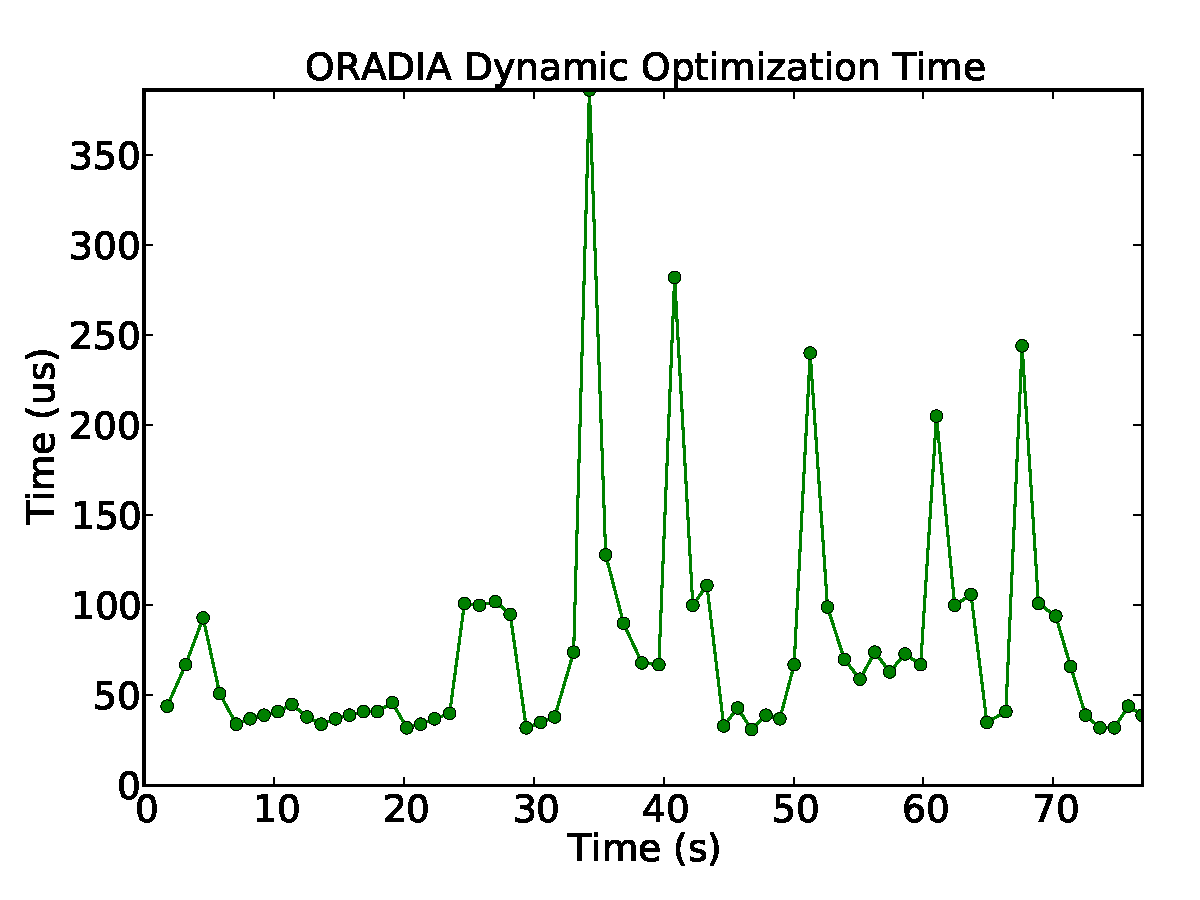
\includegraphics[bb=0 0 576 432,width=\columnwidth]{opt_time.pdf}
%%		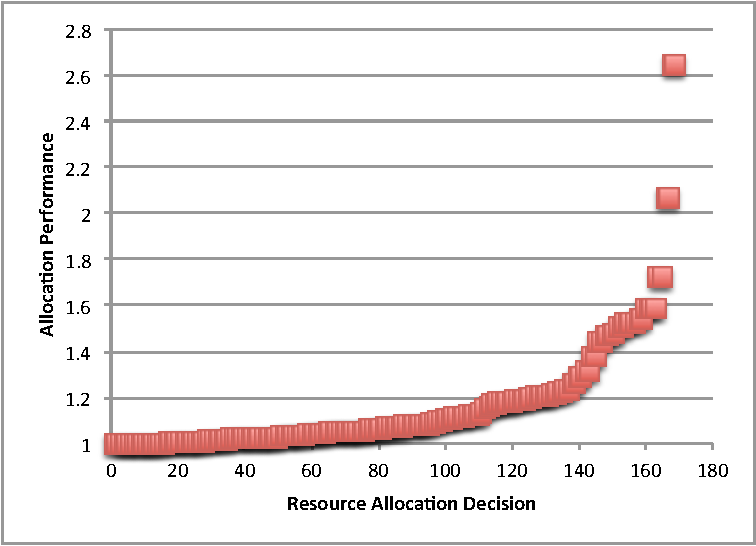
\includegraphics[width=.45\textwidth]{parsec_decision_points.pdf}
%		\caption{Performance of our penalty optimization algorithm}
%		\label{optimization_perf}
%	\end{center}
%\end{figure}


%Figure~\ref{optimization_perf} shows performance of the penalty optimization algorithm implemented in \tess.  

%For our video conferencing scenario the average runtime is \fix{x} and then worst case runtime is \fix{y}.  \fix{explain where the variance comes from}
